%!TEX root = ./main.tex

\documentclass[aspectratio=169,t,xcolor=table]{beamer}
\usepackage[utf8]{inputenc}
\usepackage{booktabs} 
\usepackage{subcaption}
\usepackage{src/stylings/main}

\usepackage[utf8]{inputenc}
\usepackage[T1]{fontenc}
\usepackage{hyperref}
\usepackage{csquotes}
\usepackage[
	backend=biber,
	style=numeric,
	citestyle=numeric,
	sorting=none,
	url=false]{biblatex}

\setbeamertemplate{bibliography item}[text]
\renewcommand*{\bibfont}{\scriptsize}
% \addbibresource{src/bib/cites.bib}
\addbibresource{src/bib/ref.bib}

\usepackage{array}
\usepackage{tabularx}
\usepackage{lipsum}
\setcounter{tocdepth}{3}

\usepackage{appendixnumberbeamer}
\usepackage{listings}
\usepackage{graphicx}
\graphicspath{{assets/}}

\title{Mapping GraphQL to the Haskell Type System}
\subtitle{Bachelor Thesis}
\institute[UHH] 
{
  University of Hamburg \\ 
  Faculty of Mathematics, Informatics and Natural Sciences (MIN) \\
  B.Sc. Human‐Computer Interaction (HCI)

}
\date{08.02.2020}
\author{Daviti Nalchevanidze}

\begin{document}
\setLogos{assets/logo/uhh.pdf}{assets/logo/uhh-compact.pdf} 
\setLayout{titlepage}
\frame[noframenumbering]{\titlepage}
\setLayout{regular} 
%!TEX root = ../../main.tex

\begin{frame}
    \frametitle{Table of Contents}
    \tableofcontents
\end{frame}
\newcommand{\importGQL}[2]{
    \lstinputlisting[
        caption={#2},
    ]{src/code/#1.gql}   
}

\newcommand{\importHS}[2]{
    \lstinputlisting[
        language={haskell},
        caption={#2},
    ]{src/code/#1.hs}   
}

\newcommand{\importHSFragment}[4]{
    \lstinputlisting[
        language={haskell},
        caption={#4},
        firstline=#2, 
        lastline=#3,
    ]{src/code/#1.hs}   
}

\newcommand{\importJSON}[2]{
    \lstinputlisting[
        language={haskell},
        caption={#2},
    ]{src/code/#1.json}   
}

\newcommand{\expr}[1]{\hspace{0.2mm}\mbox{\textcolor{green!35!blue!55!black}{\texttt{#1}}}}

\newcommand{\refGQL}[1]{Listing \ref{ls:gql:#1}}
\newcommand{\refHS}[1]{Listing \ref{ls:hs:#1}}

\newcommand{\li}[1]{\item \textcolor{black}{\textbf{#1}}:}

\section{Motivation}

\begin{frame}\frametitle{Motivation}

    \footnotesize

    \begin{alertblock}{Aktuelle Herausforderungen}
        Heute werden riesige Mengen an Informationen über das Web ausgetauscht. Dies erhöht die \alert{Wartezeit} und die \alert{Komplexität} der Anwendungen. 
    \end{alertblock}

    \begin{alertblock}{Haskell und  GraphQL}
        Die Funktionssprache Haskell und GraphQL können diese Probleme verringern.
    \end{alertblock}

    \begin{block}{Fehlende Bibliothek}
        Es gibt einige Bibliotheken, die GraphQL in Haskell implementieren, aber entweder bieten sie keine ausreichende Typsicherheit oder sie bilden GraphQL in Haskell auf sehr komplizierte Weise ab. 
    \end{block}

\end{frame}

\begin{frame}\frametitle{Zielsetzung}

    In dieser arbeit versuchen wir, eine Bibliothek bereitzustellen,
    die \alert{typensicherheit bietet} und dennoch \alert{einfach zu schreiben} ist. 
    dabei sollen folgende ziele verfolgt werden

\end{frame}
%!TEX root = ../../main.tex
\section{Background}

\subsection{Haskell}
\begin{frame}\frametitle{Haskell}

Haskell is a non-strict, purely functional language with static typing and algebraic data types. Many developers think that Haskell programs look nice~\cite{history-of-haskell}.

\begin{block}{Haskell is lazy}
    % Laziness is a primary concern in Haskell's design. 
    Haskell is a non-strict semantic language; lazy evaluation is just a technique to implement it~\cite{history-of-haskell}.
\end{block}

\begin{block}{Haskell is pure}
The lazy evaluation requires a pure design since a function call can no longer guarantee the reliable execution of the side-effects~\cite{history-of-haskell}.
\end{block}

\end{frame}

\begin{frame}\frametitle{Algebraic Data Types}

% Algebraic data types and pattern matching are fundamental to most modern functional languages~\cite{trees-that-grow}. Using pattern matching against algebraic data types improves readability significantly~\cite{history-of-haskell}.

An algebraic data type is the sum of one or more alternatives, where each alternative is a product of zero or more fields (Haskell also allows a sum of zero alternatives, the so-called empty type)~\cite{history-of-haskell}. 
        
\importHS{maybe}{Algebraic Data Types~\cite{history-of-haskell}}

Once a data type is defined and compiled, its definition cannot be extended by adding new data constructors or new fields~\cite{trees-that-grow}.

\end{frame}

\begin{frame}\frametitle{Records }

The record system provides syntactic sugar for what might otherwise be written using ordinary, positional, algebraic data type declarations~\cite{lw-ext-records}. 

\importHSFragment{records}{0}{4}{Haskell Record}

Haskell record are not extensible. There are no operators for adding and removing fields in a record, we cannot reuse labels between different record types~\cite{poly-ext-records, hlist,lw-ext-records}. 

\end{frame}

\begin{frame}\frametitle{Record Values}

Records bring significant advantages and greatly simplify programming with data structures that have many components. Since the individual components are accessed by name (not by position), the fields' ordering is not crucial~\cite{lw-ext-records}.

\importHSFragment{records}{6}{10}{Haskell Record Values}
% For example, 
% the data type Deity declares a regular algebraic data type, but at the same time, constructor field accessors and modifiers. 

\end{frame}

% \begin{frame}\frametitle{Monads}

% Haskell abstracts side effects with monads. monads are formed by a type constructor \expr{M} and a pair of functions, \expr{return} and \expr{>>=}~\cite{history-of-haskell,essence-of-fp}. The type \expr{M a} is a computation that returns a value of type \expr{a} and possibly performs some side effects~\cite{history-of-haskell}. The purpose of \expr{return} and \expr{>>=} is to push a value into computation and to evaluate a computation, yielding a value~\cite{essence-of-fp}.

% Since the monad allows the compiler to determine impure and pure operations, the Haskell language can use specific optimizations. However, the developer still has the freedom to define their execution order~\cite{history-of-haskell}.

% \end{frame}

\begin{frame}\frametitle{Datatype-Generic Programming}
    
Datatype-generic programming enables writing single functions that address various cases and types.~\cite{derivable-type-classes}. 
It increases program reliability, reduces code duplication, while guaranteeing safety~\cite{datatype-generic-programming,optimizing-generics}.

\importHS{generics}{Generic Deriving}
    
The generic derivation represents all types and values by generic representation types. The user can convert any types to their generic representation, operate on them, and convert them back to their original types~\cite{optimizing-generics, ghc-generics}.

\end{frame}
\subsection{GraphQL}

\begin{frame}\frametitle{GraphQL}

  \footnotesize
  \begin{block}{What is GraphQL?}
  GraphQL is an application layer framework for solving the efficiency problems of web communication~\cite{gql-iot}. It was developed internally at  Facebook for three years and published in 2016~\cite{initial-analysis-of-gql}. 
  \end{block}

  \begin{block}{GraphQL as current trend}
  Since its first appearance, it has gained a rich open-source ecosystem~\cite{gql-healthcare}, and the trust of companies from various sectors. e.g. (GitHub), entertainment (Netflix), finance (PayPal), travel (KLM), and others~\cite{morph-gql-1}.
  \end{block}

\begin{block}{Typed Query Language}
  GraphQL is a hierarchically structured language with a strongly typed schema~\cite{gql-healthcare}, where the type system (as a public schema) provides a solid contract between client and server and the possibility of errors caused by a part of the invalid request on the client~\cite{real-time-sys-arc-based-on-gql}.
\end{block}

\end{frame}

\begin{frame}\frametitle{Advantages and Disadvantages of GraphQL}

\footnotesize

\begin{block}{Over-Fetching and Under-Fetching}

reduces the number of JSON responses returned by API calls. which interesting for mobile applications, often faced with limited bandwidth and speed~\cite{migrating-to-gql,gql-healthcare}. In the studies showed that GraphQL could significantly improve performance by reducing unnecessary transfer costs and resulted in a significant reduction in energy consumption and transaction delays and even a reduction in response size~\cite{migrating-to-gql,real-time-sys-arc-based-on-gql,gql-iot}.
\end{block}

\begin{block}{API Versioning}

a stable and consistent contract between two systems for information exchange while remaining flexible for future changes~\cite{gql-healthcare}. 

\begin{itemize}
  \item new fields added to a type do not result in client changes~\cite{migrating-to-gql}. 
  \item provides an \expr{@deprecated} annotation for unsupported fields~\cite{migrating-to-gql}. 
\end{itemize}

\end{block}

\begin{block}{Facilitates Rapid Product Development}

GraphQL requires less effort to implement requirements than REST~\cite{rest-vs-gql-controlled-experiment}.

\begin{itemize}
  \item  GraphQL uses familiar syntax and semantics, similar to common programming languages, shortening the learning curve for beginners~\cite{rest-vs-gql-controlled-experiment}.
  \item GraphQL-IDEs enables real-time query validation and auto-completion~\cite{rest-vs-gql-controlled-experiment,migrating-to-gql}.
  \item Introspection frees up servers to support an interface description language and enables clients to explore the REST instantly~\cite{migrating-to-gql}. 
\end{itemize}

\end{block}

% Using GraphQL with Haskell has the following advantages: First, the languages are typed and support union types. Second, GraphQL fields are lazy, concurrent, resolvable functions that fit Haskell's non-strict and concurrent nature~\cite{gql-spec,haskell-homepage}. This way, the developer does not worry about laziness and concurrency and focuses on business logic.


\end{frame}

\begin{frame}\frametitle{Language}

\begin{block}{GraphQL Schema}

GraphQL allows the client to query a domain-specific database represented by a schema. The schema can be defined with a domain-specific language called Schema Definition Language (SDL)~\cite{migrating-to-gql,gql-on-graph-db}.

\importGQL{schema}{Schema}

\end{block}

\begin{block}{GraphQL Queries}

GraphQL provides a query language that is used by clients. Every GraphQL query is defined in this language and sent to the single GraphQL endpoint as a simple string~\cite{migrating-to-gql,real-time-sys-arc-based-on-gql}.
The query is syntactically similar to JSON but follows the server's specific schema instead of arbitrary JSON objects~\cite{gql-on-graph-db,initial-analysis-of-gql}. 

\importGQL{query}{Sample GraphQL Query Using the Mythology }

To respond to queries, the developer of a GraphQL server must implement a function for each field of type resolver. These functions return query values from an underlying data structure.  The GraphQL engine calls them during the query and returns their value as a JSON document~\cite{migrating-to-gql,real-time-sys-arc-based-on-gql}. 

\importJSON{response}{GraphQL Response of the Query}

\end{block}

\end{frame}



\section{Requirements}

\begin{frame}\frametitle{Requirements}  

\begin{itemize}
    \li{Maintainability} a Maintainable software can adapt to continuous changes.
    \begin{itemize}
        \item Low boilerplate
        \item Familiarity
        \item Modularity
    \end{itemize}
    \li{Reliability} We aim to avoid runtime failures. 
    \begin{itemize}
        \item Type safety    
        \item Compliance with GraphQL specifications
    \end{itemize}
    \li{Efficiency} The library must be lazy and efficient.
\end{itemize}

\end{frame}
\section{Library}

\subsection{Architecture Overview}

\begin{frame}\frametitle{Architecture Overview}

%!TEX root = ../../main.tex

\begin{figure}
\caption{
    Dependency Graph of the Morpheus GraphQL Packages
    \label{fig:dependency-graph}
    }
\begin{center}
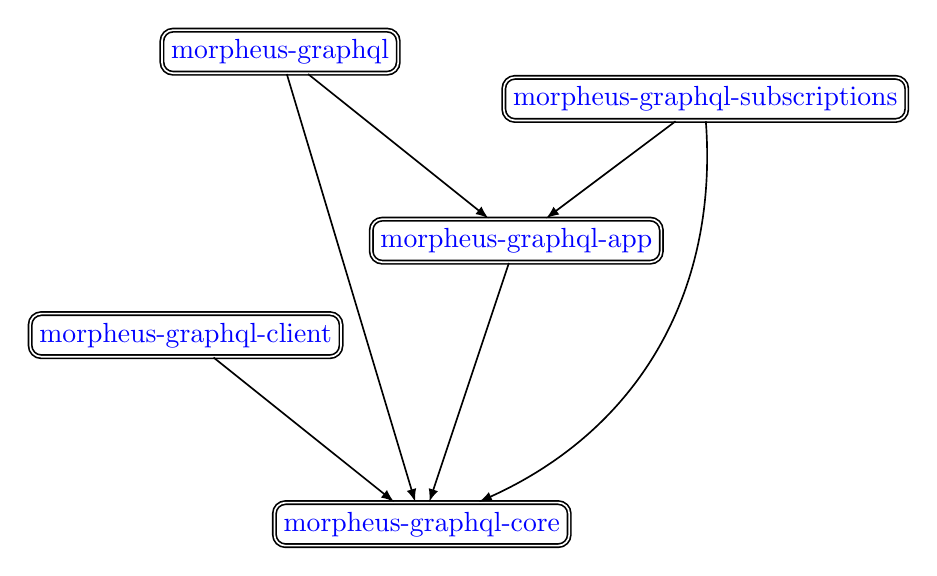
\begin{tikzpicture}[
        scale=.6,
        auto=left,
        -latex ,
        auto ,
        node distance =2 cm and 2cm ,
        % on grid ,
        semithick ,
        package/.style ={ fill=red!20,draw,double,rounded corners ,top color =white ,draw , text=blue , minimum width =1 cm},
    ] 
    \node[package] (core) at (10,0) {morpheus-graphql-core};
    \node[package] (client) at (5,4)  {morpheus-graphql-client};
    \node[package] (app) at (12,6)  {morpheus-graphql-app};
    \node[package] (server) at (7,10)  {morpheus-graphql};
    \node[package] (subs) at (16,9) {morpheus-graphql-subscriptions};
  
    \path (client) edge (core);
    \path (app)  edge (core);
    \path (server)  edge  (core);
    \path (server)  edge  (app);
    \path (subs)  edge  (app);
    \path 
        (subs) 
            edge [bend left =35] 
        (core);  

\end{tikzpicture}
\end{center}
\end{figure}

\end{frame}

%!TEX root = ../../main.tex

\subsection{Design Decisions} 

\begin{frame}\frametitle{Design Decisions}

\begin{itemize}
    \li{Code-First Approach} A single type change automatically updates the resolver types and GraphQL schema, simplifying maintenance. 
    \li{Embeded Domain Specific Language} By using the familiar syntax of the native language, users can focus on domain-specific problems~\cite{edsl-modeling}.
    \li{Datatype-Generic Programming}datatype-generic programming eliminates boilerplate code~\cite{scrap-your-boilerplate}.
    \li{Monadic Resolvers} Since all side effects in Haskell are performed with monads, field resolvers will be monadic functions. 
    \li{Parameterized Resolver Types} Parametric polymorphism allows the modular definition of resolver types, where the type parameter determines the allowed operations.
\end{itemize}
\end{frame}

\subsection{Schema Derivation} 
\begin{frame}\frametitle{Schema Derivation}

GraphQL models the schema as a graph, where nodes are types and fields are edges. The graph starts with a root node that branches to API-specific types~\cite{migrating-to-gql}.  We use deep-first search and derive all schema types from the root node. We also use cycle checking to avoid looping on cycles.

\end{frame}

%!TEX root = ../../../main.tex

\subsection{Mapping Rules}

\begin{frame}\frametitle{Mapping Built-in Types}
\begin{itemize}
  \li{Wrapping Types}
  \begin{itemize}
    \li{Non-Null} inverse mapping with Maybe
    \li{List} List
  \end{itemize}
  \li{Scalar Types}
  \begin{itemize}
    \li{Int} Int
    \li{Float} Double
    \li{String} Text
    \li{Boolean} Bool
    \li{ID}  defined custom data type ID 
  \end{itemize}
\end{itemize}
\end{frame}

\begin{frame}\frametitle{Mapping Enums}

enum types describe the set of possible independent, unique values~\cite{gql-spec}.

\importHS{enum}{GraphQL Enum in Haskell}

\importGQL{enum}{GraphQL Enum}

\end{frame}

\begin{frame}\frametitle{Mapping Input Object And Field Arguments}

A GraphQL input objects and arguments are is a sets of labeled input values~\cite{gql-spec}. They resemble single constructor Haskell records. 

\importHS{input-object}{GraphQL Input Object in Haskell}
\importGQL{input-object}{Input Object Deity}

\end{frame}
\begin{frame}[allowframebreaks]\frametitle{Mapping Objects}

GraphQL objects are a set of named fields, where fields themselves consist of argument and return type~\cite{gql-spec}. We represent the object types with parameterized records, where the record fields can take function types. This technique allows types to be defined independently of the resolver operations, and the concrete operations can be passed recursively from parent to child. 

\importHS{object-type}{GraphQL Object in Haskell}

\importGQL{object-type}{GraphQL Object in Haskell}

\end{frame}

\begin{frame}[allowframebreaks]\frametitle{Unions}

GraphQL unions represent an object, one of the possible alternative object types, but do not provide guaranteed fields between them~\cite{gql-spec}. 

% While in GraphQL, we only refer to the object type in the list of possible types, in Haskell, we put each of them into a specific constructor. Furthermore, in Haskell, we can create alternative objects only with constructors without defining their types.

\importHS{union}{Union Types}
\begin{itemize}
  \item we unpack constructors, where the name is the concatenation of the type constructor name and the referencing type name. for rest we generate new constructors object.
  \item since GraphQL does not supports empty objects we add every empty object unit field.
\end{itemize}

\importGQL{union}{Union Types}

\end{frame}

% \begin{frame}\frametitle{Determining GraphQL Types in Haskell}
% Compiler applies the following rules with a given execution order to achieve deterministic derivation.
% \begin{enumerate}
%   \li{Scalar, Wrapper, Interface} Derive scalar, wrapper, interface if the type has explicitly specified associated kinds. 
%   \li{Field Arguments} Derive field arguments if the type is used as an argument of the object field. 
%   \li{Enum} Derive enum if all data type constructors are empty.
%   \li{Object} Derive object if the type has a single non-empty constructor, and its parent \footnote{Type A is the parent type of type B if it has a field that refers to type B} is Object or Union. 
%   \li{InputObject} Derive input object if the type has a single non-empty constructor, and its parent is InputObject or Field Arguments.
%   \li{Union} Derive Union if the type has multiple constructors and its parent is Object or Union.
%   \li{Fail} All other types are not supported.
% \end{enumerate}
% \end{frame}

\section{Evaluation}

\begin{frame}[allowframebreaks]\frametitle{Evaluation}

\begin{block}{Maintainability}

  \begin{itemize}
  
    \li{Low Boilerplate and Familiarity} The library follows a code-first approach and and derives api from native Haskell types based on data-type-generic programming. the approach is familiar reduces boilerplate and improves maintainability.

    \li{Modularity}
      The library architecture divides functionalities into separate, coherent packages. 
    
      The modularity of the API definition is achieved by introducing parameterized resolver types. They decouple the types from the accessible operations, and thus one can use one data type for different operations.

  \end{itemize}

\end{block}


\begin{block}{Reliability}

\begin{itemize}

  \li{Type Safety} 
    \begin{enumerate}

      \li{Deterministic deriving} The mapping rules cover all Haskell algebraic data types.

      \li{Resolver validity} The Haskell compiler reports any value mismatch at compile time.
      
      \li{Schema validity} Haskell and GraphQL adopt different types of type systems. That why the Haskell compiler cannot check the validity of all GraphQL-specific rules. Therefore, to ensure schema validity, we provide the function \expr{compileTimeSchemaValidation}, which takes the \expr{RootResolver} type signature and fails if the schema is invalid.
    
    \end{enumerate}

  \li{Complience with GraphQL Specifications} The library meets all the critical parts of the specifications. However, there are also small deviations in favor of flexibility, e.g., the use of \expr{Int} instead of \expr{Int32}. Moreover, interfaces and directives are still not fully implemented. 

\end{itemize}

\end{block}

\begin{block}{Efficiency} we used the type \expr{Text} instead of \expr{String}. the library only executes the resolvers necessary for the query. The library is extensible with Haxl, which allows efficient reuse of resolvers without running into the n+1 selects problem.

\end{block}

\end{frame}

\begin{frame}\frametitle{General Overview}

Our prototype meets our predefined requirements, with an acceptable tradeoff between flexibility and compliance. We provide a straightforward approach to GraphQL API definitions while still guaranteeing type safety. Besides, users can achieve efficiency in the combination of Morpheus GraphQL and Haxl, as GraphQL solves over-fetching and under-fetching problems for a client and  Haxl for the backend.

Nevertheless, we run into some limitations: First, Haskell permits different naming of values and types than GraphQL. Second, sets and non-empty collections cannot be modeled in GraphQL because it provides only list types for collections. Therefore, sets and non-empty collections are represented to GraphQL clients with regular lists, and the client cannot check the validity of input values at compile time. Third, since Haskell makes no distinction between input and output types, mapping Haskell types requires support for input unions, which is not supported by GraphQL. Fourth, Haskell does not provide interfaces, so we do not yet have a satisfying way to support them. 
\end{frame}

\section{Conclusions}

\begin{frame}\frametitle{Advantages}

The presented approach successfully implements the requirements and provides:

\begin{itemize}
    \item easy-to-use interface while ensuring type safety.
    \item We preferred intuitive design over extensibility.
    \item The library can be learned quickly by beginners.
    \item Importing schemas from SDL facilitates quick starts and migration from other languages.
    \item A type-safe client package allows developers to implement entire applications in one language or even query data for resolvers from other GraphQL servers.
    \item \expr{Apps} are members of the type class semigroup and can be composed.
\end{itemize}

\end{frame}

\begin{frame}\frametitle{Limitations}

\begin{itemize}
    \item Haskell permits different naming of values and types than GraphQL. 
    \item sets and non-empty collections cannot be modeled in GraphQL because it provides only list types for collections. 
    \item mapping Haskell types requires support for input unions, which is not supported by GraphQL. 
    \item Haskell does not provide interfaces, so we do not yet have a satisfying way to support them. 
\end{itemize}

\end{frame}

\begin{frame}\frametitle{Outlook}

\begin{itemize}
    \li{Support Interfaces} representation of interfaces with "type guards" on unions. 
    \li{Type-Level Curried Arguments} flexible argument definitions for a small number of arguments than our current approach since the user does not have to define a new data type for each field. 
    \li{Custom Collections} Since GraphQL has only one type (List) for collections, we cannot represent collections with certain constraints. 
    \li{Support Directives}Since the GraphQL specification does not specify a particular implementation strategy for directives, it is up to each server library to provide a suitable API~\cite{schema-directives}.
    \li{Support Input Unions} GraphQL does not support input unions. While this function's value is essentially understood, its implementation is not cleared~\cite{gql-spec-input-unions}. 

\end{itemize}

\end{frame}

\section{Contributions}

\begin{frame}\frametitle{Contributions}

\begin{itemize} 
  
    \li{@Pygmalion} initial name and inspirations

    \li{@krisajenkins} Parser optimization, parameterized resolver types
    
    \li{@theobat} custom wrapping types and the library Massalia

\end{itemize}

\end{frame}
%!TEX root = ../main.tex
\section{Examples}

\begin{frame}\frametitle{Morpheus}

repository: \url{https://github.com/nalchevanidze/morpheus-haxl-example}

\end{frame}
\setLayout{blank}
%!TEX root = ../../main.tex

\section*{Thanks}
\setBGColor{white}
\begin{frame}
    
    \centering
    \vspace{2cm}
    
    \textbf{\Huge Danke!}
 
    \ \\
    \ \\
    \textbf{Fragen oder Anregungen?}
    
    \text{\footnotesize d.nalchevanidze@gmail.com}
    
    \vspace{1.5cm}
    \begin{figure}
        \centering
        \begin{subfigure}{0.2\textwidth}
            \centering\pgfuseimage{logo_title}
        \end{subfigure}%      
    \end{figure}
\end{frame}
\setLayout{titlepage}
\titlepage
\setLayout{regular} 

\begin{frame}[plain, noframenumbering,allowframebreaks]{References}
    \printbibliography
\end{frame}

\end{document}